\section{Anforderungen höherer Programmiersprachen}
\label{sec:anforderungen}

\textbf{Begriffe}:
\begin{items}
  \item \underline{Maschinensprache}: Für Prozessor verständliche Anweisungsrepräsentation, z.B. \code{00101101001110101}
  \item \underline{Assemblersprache}: Für Menschen verständliche Maaschinensprache, z.B. \code{add \$s2, \$s1, \$s0}
  \item \underline{Assembler}: Übersetzt Assemblersprache eindeutig in Maschinensprache
  \item \underline{Objektcode}: Maschinenprogramm mit ungelösten externen Referenzen
  \item \underline{Binder/Linker}: Löst ungelöste Referenzen auf, verbindet alles zu einem ausführbaren Maschinenprogramm
\end{items}
\begin{figure}[ht]
  \centering
  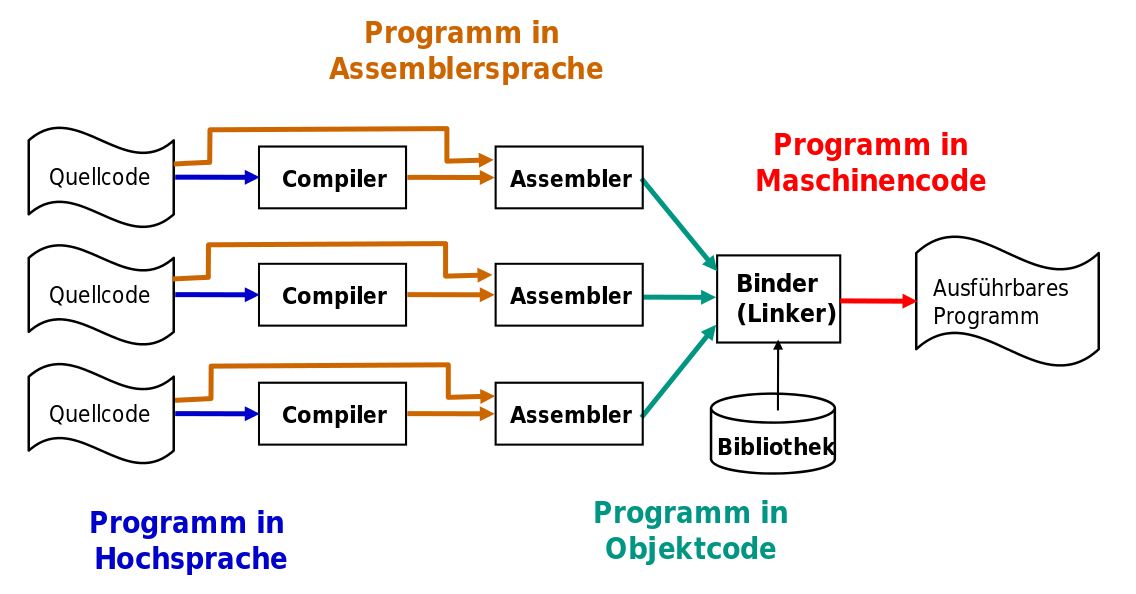
\includegraphics[width=0.33\textwidth]{QuellcodeZuProgramm}
  \label{QuellcodeZuProgramm}
\end{figure}

\textbf{Programmiersprache C}:
\begin{items}
  \item Zwischenstellung zwischen Assembler und Hochsprache
  \item hohe Portabilität trotz guter Architekturanpassung
  \item einfache Programmierung
  \item \underline{Datentypen}: \code{char, int, float, double}
  \item \underline{Kontrollstrukturen}: Entscheidungen, Schleifen, Blöcke, Unterprogramme
  \item \underline{Zeiger} als Parameter möglich
\end{items}
\begin{figure}[ht]
  \centering
  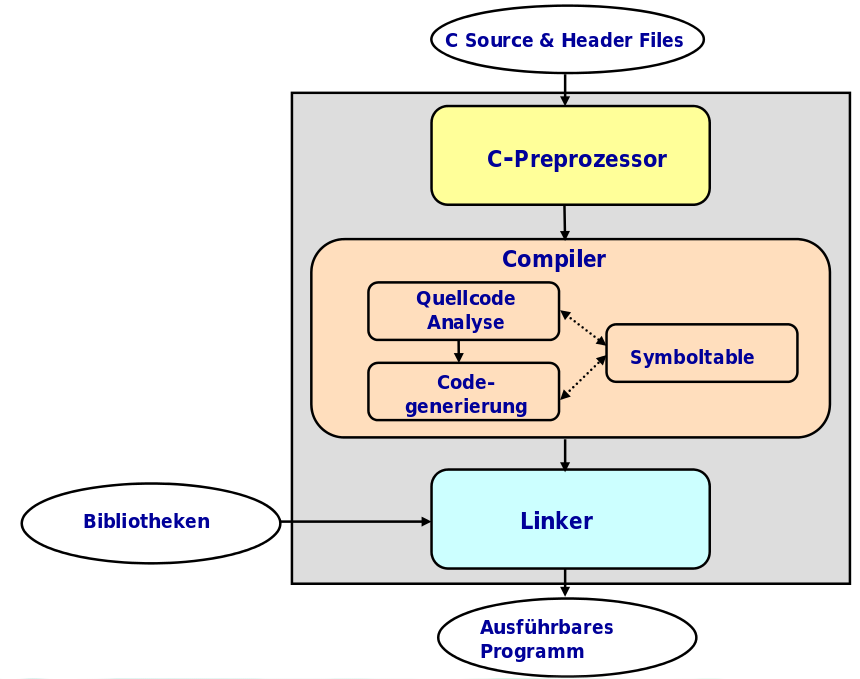
\includegraphics[width=0.33\textwidth]{CWorkflow}
  \label{CWorkflow}
\end{figure}

\newpage

\textbf{C - Datentypen}:
\begin{items}
  \item \underline{\code{char}}: Ein Zeichen, meist 1 Byte
  \item \underline{\code{int}}: Integerzahl, 2 oder 4 Byte
  \item \underline{\code{float}}: Gleitkommazahl, meist 4 Byte
  \item \underline{\code{double}}: Gleitkommazahl, meist 8 Byte
\end{items}

\textbf{C - Operatoren}:
\begin{items}
  \item \underline{\code{*}}: Multiplikation (\code{x*y})
  \item \underline{\code{/}}: Division (\code{x/y})
  \item \underline{\code{\%}}: Modulo (\code{x\%y})
  \item \underline{\code{+}}: Addition (\code{x+y})
  \item \underline{\code{-}}: Subtraktion (\code{x-y})
  \item \code{+} und \code{-} auch als Prä- und Postfix, alle auch als assign (\code{=} anhängen)
\end{items}

\textbf{C - Bit-Operatoren}:
\begin{items}
  \item \underline{\code{\~}}: Bitweise NOT (\code{\~x})
  \item \underline{\code{<<}}: links schieben (\code{x<<y})
  \item \underline{\code{>>}}: rechts schieben (\code{x>>y})
  \item \underline{\code{&}}: bitweise AND (\code{x&y})
  \item \underline{\code{^}}: bitweise XOR (\code{x^y})
  \item \underline{\code{|}}: bitweise OR (\code{x|y})
  \item alle auch als Assign (\code{=} anhängen)
\end{items}

\textbf{C - Vergleichsoperatoren}:
\begin{items}
  \item \underline{\code{>,<}}: größer, kleiner als (\code{x>y, x<y})
  \item \underline{\code{>=,<=}}: größergleich, kleinergleich als (\code{x>=y, x<=y})
  \item \underline{\code{==,!=}}: gleich, ungleich (\code{x==y, x!=y})
\end{items}

\textbf{C - Spezialoperatoren}:
\begin{items}
  \item \underline{Auswahloperator}: \code{z = (a < b) ? a : b} (\code{z=a}, falls \code{a<b}, sonst \code{z=b})
\end{items}